\section{AI流程图}


AI帮助绘制流程图具有重要意义。它不仅能够显著节省时间,还能提升绘制的准确性和效率。通过自然语言描述,AI工具可以快速生成流程图的基本框架,用户只需输入简单的指令,如“开始”“决策点”“流程步骤”等,AI就能自动识别并绘制相应的图形和连接线。此外,AI还能根据上下文智能识别关键节点和流程关系,即使用户提供的信息不完整,也能推测出合适的步骤。AI工具还能自动调整图形布局和连接线,使流程图更加整洁美观,同时支持实时更新与修改,确保流程图的连贯性和一致性。这种智能化的绘图方式不仅适用于企业管理、项目规划、技术开发等复杂场景,还能帮助个人高效地制定学习计划或整理思维导图,极大地提升了工作效率和质量。


\textbf{案例:历史进程流程图}。本案例旨在梳理``丝绸之路文化交流''中的技术传播路径。下面给出与AI交流过程。

\prompt{``用Mermaid语法绘制佛教从印度经中亚传入中国的流程图,包含主要节点和传播方式''}
  
\begin{gptbox}
\small{
\begin{lstlisting}[language=Markdown]
    graph LR
    A[印度那烂陀寺] -->|法显陆路取经| B[龟兹]
    B --> C[敦煌莫高窟]
    A -->|海上丝绸之路| D[广州光孝寺]
    C --> E[长安大雁塔]
    D --> E
\end{lstlisting}
}
\end{gptbox}


最后,将代码粘贴至Markdown编辑器或Mermaid Live Editor,立即生成矢量图,如\reffig{fig:flow-chart}所示。

\fig[h]{
    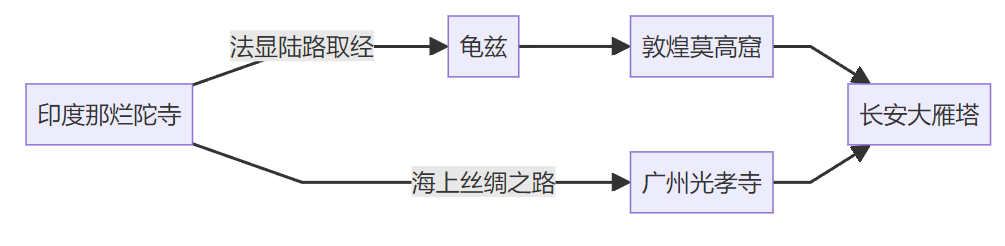
\includegraphics[width=0.7\textwidth]{assets/figures/1739189207681.jpg} %插入图片,[]中设置图片大小,{}中是图片文件名
    \caption{矢量图} %最终文档中希望显示的图片标题
    \label{fig:flow-chart} %用于文内引用的标签
}
\end{enumerate}